\PassOptionsToPackage{unicode=true}{hyperref} % options for packages loaded elsewhere
\PassOptionsToPackage{hyphens}{url}
%
\documentclass[12pt,english,]{article}
\usepackage{lmodern}
\usepackage{amssymb,amsmath}
\usepackage{ifxetex,ifluatex}
\usepackage{fixltx2e} % provides \textsubscript
\ifnum 0\ifxetex 1\fi\ifluatex 1\fi=0 % if pdftex
  \usepackage[T1]{fontenc}
  \usepackage[utf8]{inputenc}
  \usepackage{textcomp} % provides euro and other symbols
\else % if luatex or xelatex
  \usepackage{unicode-math}
  \defaultfontfeatures{Ligatures=TeX,Scale=MatchLowercase}
\fi
% use upquote if available, for straight quotes in verbatim environments
\IfFileExists{upquote.sty}{\usepackage{upquote}}{}
% use microtype if available
\IfFileExists{microtype.sty}{%
\usepackage[]{microtype}
\UseMicrotypeSet[protrusion]{basicmath} % disable protrusion for tt fonts
}{}
\usepackage{hyperref}
\hypersetup{
            pdfborder={0 0 0},
            breaklinks=true}
\urlstyle{same}  % don't use monospace font for urls
\usepackage[margin=1in]{geometry}
\usepackage{graphicx,grffile}
\makeatletter
\def\maxwidth{\ifdim\Gin@nat@width>\linewidth\linewidth\else\Gin@nat@width\fi}
\def\maxheight{\ifdim\Gin@nat@height>\textheight\textheight\else\Gin@nat@height\fi}
\makeatother
% Scale images if necessary, so that they will not overflow the page
% margins by default, and it is still possible to overwrite the defaults
% using explicit options in \includegraphics[width, height, ...]{}
\setkeys{Gin}{width=\maxwidth,height=\maxheight,keepaspectratio}
\setlength{\emergencystretch}{3em}  % prevent overfull lines
\providecommand{\tightlist}{%
  \setlength{\itemsep}{0pt}\setlength{\parskip}{0pt}}
\setcounter{secnumdepth}{0}
% Redefines (sub)paragraphs to behave more like sections
\ifx\paragraph\undefined\else
\let\oldparagraph\paragraph
\renewcommand{\paragraph}[1]{\oldparagraph{#1}\mbox{}}
\fi
\ifx\subparagraph\undefined\else
\let\oldsubparagraph\subparagraph
\renewcommand{\subparagraph}[1]{\oldsubparagraph{#1}\mbox{}}
\fi

% set default figure placement to htbp
\makeatletter
\def\fps@figure{htbp}
\makeatother

\usepackage{float}
\usepackage[boxruled,vlined]{algorithm2e}
\usepackage{listings}
\usepackage{xcolor}
\usepackage {tikz}
\usepackage{indentfirst}
\usepackage{tabularx}
\usepackage{multirow}
\usepackage{pgfplots}
\usepackage{wrapfig}
%\usepackage[bottom]{footmisc}
\colorlet{mygray}{black!30}
\colorlet{mygreen}{green!60!black}
\colorlet{mymauve}{red!90}

\lstset{
  tabsize=2,
  backgroundcolor=\color{gray!10},  
  basicstyle=\ttfamily,
  columns=fullflexible,
  breakatwhitespace=false,      
  breaklines=true,                
  captionpos=b,                    
  commentstyle=\color{mygreen}, 
  extendedchars=true,              
  frame=single,                   
  keepspaces=true,             
  keywordstyle=\bfseries\color{blue},      
  language=c++,                 
  numbers=left,                
  numbersep=5pt,
  breaklines=true,
  numberstyle=\tiny, 
  rulecolor=\color{mygray},        
  showspaces=false,               
  showtabs=true,                                  
  stringstyle=\color{mymauve},                          
  title=\lstname                
}

\definecolor{light-gray}{gray}{0.9}
\newcommand{\code}[1]{\colorbox{light-gray}{\texttt{#1}}}
\newcommand{\pnt}[1]{{\scriptstyle#1}}
\let\origfigure\figure
\let\endorigfigure\endfigure
\renewenvironment{figure}[1][2] {
    \expandafter\origfigure\expandafter[H]
} {
    \endorigfigure
}
\usepackage{etoolbox}
\makeatletter
\providecommand{\subtitle}[1]{% add subtitle to \maketitle
  \apptocmd{\@title}{\par {\large #1 \par}}{}{}
}
\makeatother
\ifnum 0\ifxetex 1\fi\ifluatex 1\fi=0 % if pdftex
  \usepackage[shorthands=off,main=english]{babel}
\else
  % load polyglossia as late as possible as it *could* call bidi if RTL lang (e.g. Hebrew or Arabic)
  \usepackage{polyglossia}
  \setmainlanguage[]{english}
\fi

\title{\textbf{Project Report}\\
\Large{Implementation of Finger Search:}}
\providecommand{\subtitle}[1]{}
\subtitle{An Extended Feature of Some Data Structures}
\author{Minh Thang Cao}
\date{24 February 2021}

\begin{document}
\maketitle

\graphicspath{ {./} }

\hypertarget{section1}{%
\section{\texorpdfstring{1
\enspace Introduction}{1 Introduction}}\label{section1}}

Finger Search is an extended feature, which is suitable for some popular
data structures, that improves the running time of search operations as
well as other ones that depend on searching. Finger Search uses a
pointer to an element, called \emph{finger}, in the data structure to
reduce the length of search path. Instead of searching from a normal
start point, Finger Search starts at the \emph{finger}. Let \(d\) be the
difference between ranks\footnote{Denoted \(i\) if \(x\) is the
  \(i^{th}\) smallest element in the data structure (consistent with
  only smallest or largest for all elements)} of the \emph{finger} and
the target value, the running time of Finger Search is proportional to
\(d\).

\hypertarget{section2}{%
\section{\texorpdfstring{2 \enspace Finger Search on
Treaps}{2 Finger Search on Treaps}}\label{section2}}

Briefly, Treap is a Randomized Binary Search Tree which is a combination
of Binary Search Tree and Heap. Each nodes in Treap holds a randomized
priority which is used to maintain the Heap properties. The nodes order
in a Treap satisfies ascending values in an inorder traversal while
their priority satisfies min-heap (or max-heap) property, in which
priority of a node is always smaller (or larger) than its children. This
randomized combination creates an property of Treap that the
\emph{expected} height of a Treap is \(O(logn)\) (not always), with
\(n\) is the total number of nodes. Therefore, it supports searching and
some associated operations in expected \(O(logn)\) time which is
standard for most balanced trees. Since Finger Search produces an
expected running time, Treap is a very suitable randomized data
structure for Finger Search.

In this section, Finger Search on Treaps will be introduced along with
my implementation. Due to R. Seidel and C.R. Aragon (see \cite{1}),
there are several ways to achieve the running time proportional to the
distance \(d\) such as using multiple pointers, multiple keys, or even
without anything by relying on the shortness of the search path, and
these approaches all give us the \(O(logd)\) expected running time.
Since if we do Finger Search without any assistance of other elements,
the excess path in some cases may be much longer compared to the path
that we are supposed to search on. To minimize the probability that we
get these cases, multiple extra pointers are definitely useful, which is
used in my implementation.

\begin{wrapfigure}{r}{0.4\textwidth}
\centering
\begin{minipage}{0.35\textwidth}
\vspace{1mm}
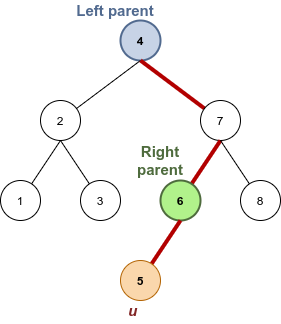
\includegraphics[width=\textwidth]{Tree.png}
\caption{\label{fig1:figs}Visualization of \textit{left parent} and \textit{right parent} of a node $u$ in a Binary Tree.}
\end{minipage}
\end{wrapfigure}

Based on what R. Seidel and C.R. Aragon found (see Section 5.4 of
\cite{1}), denote a \emph{left parent} or a \emph{right parent} of a
node \(u\) is the first ancestor of \(u\) on the path from \(u\) to the
\emph{root} node that satisfies \(u\) is on the ancestor's right or left
subtree, respectively (see Figure \ref{fig1:figs}).

\newpage
\begin{thebibliography}{9}
\bibitem{1}
Seidel, R., Aragon, C.R. Randomized search trees. \emph{Algorithmica} 16, 464–497 (1996). \url{https://doi.org/10.1007/BF01940876}

\end{thebibliography}

\end{document}
